\chapter{Programming MCB1700}
\section {The Thumb-2 Instruction Set Architecture}
The Cortex-M3 supports only the Thumb-2 (and traditional Thumb) instruction set.
With support for both 16-bit and 32-bit instructions in the Thumb-2 instruction
set, there is no need to switch the processor between Thumb state (16-bit instructions) and ARM state (32-bit instructions). 

In the RTOS lab, you will need to program a little bit in the assembler language. We introduce a few assembly instructions that you most likely need to use in your project in this section.

The general formatting of the assembler code is as follows:
\begin{eqnarray*}
    \mathtt{label} &~ &~ \\
     ~    & ~& \mathtt{opcode ~operand1, ~operand2,} ~\ldots~ ; ~  Comments
\end{eqnarray*}
The $\mathtt{label}$ is optional. Normally the first operand is the destination of the operation (note $\mathtt{STR}$ is one exception). 

Table \ref{tb_asm_instr} lists some assembly instructions that the RTX project may use. For complete instruction set reference, we refer the reader to Section 34.2 (ARM Cortex-M3 User Guide: Instruction Set) in \cite{nxp.lpc17xx.manual}.

\begin{table}
\begin{center}
\footnotesize
\begin{tabular}{lll}
\hline
Mnemonic & Operands/Examples & Description \\ \hline
$\mathtt{LDR}$ & $\mathit{Rt, [Rn, \#offset]}$ & Load Register with word \\
               & $\mathtt{LDR~ R1, [R0, \#24]}$ 
               & Load word value from an memory address R0+24 into R1\\ \hline
$\mathtt{LDM}$ & $\mathit{Rn \{!\}, reglist}$ & Load Multiple registers \\
        & $\mathtt{LDM~ R4, \{R0-R1\}}$   
        &  Load word value from memory address R4 to R0, increment the\\ 
       &&  address, load the value from the updated address to R1. \\ \hline
$\mathtt{STR}$ & $\mathit{Rt, [Rn, \#offset]}$ & Store Register word \\ 
        & $\mathtt{STR~ R3, [R2, R6]}$  
        & Store word in R3 to memory address R2+R6\\
        & $\mathtt{STR~ R1, [SP, \#20]}$
        & Store word in R1 to memory address SP+20 \\ \hline
$\mathtt{MRS}$ & $\mathit{Rd, spec\_reg}$ & Move from special register to general register \\
        & $\mathtt{MRS~ R0, MSP}$ & Read MSP into R0 \\ 
        & $\mathtt{MRS~ R0, PSP}$ & Read PSP into R0 \\ \hline
$\mathtt{MSR}$ & $\mathit{spec\_reg, Rm}$&  Move from general register to special register\\
        & $\mathtt{MSR~ MSP, R0}$ & Write R0 to MSP\\ 
        & $\mathtt{MSR~ PSP, R0}$ & Write R0 to PSP\\ \hline 
$\mathtt{PUSH}$ & $\mathit{reglist}$ & Push registers onto stack\\
        & $\mathtt{PUSH~\{R4-R11, LR\}}$ & push in order of decreasing the register numbers \\ \hline 
$\mathtt{POP}$ & $\mathit{reglist}$ & Pop registers from stack\\ 
        & $\mathtt{POP~\{R4-R11, PC\}}$ & pop in order of increasing the register numbers \\ \hline 
$\mathtt{BL}$ & $\mathit{label}$ & Branch with Link \\  
        & $\mathtt{BL~ funC}$
        & Branch to address labeled by funC, return address stored in LR\\ \hline
$\mathtt{BLX}$ & $\mathit{Rm}$ & Branch indirect with link \\
        & $\mathtt{BLX~ R12}$
        & Branch with link and exchange (Call) to an address stored in R12 \\ \hline
$\mathtt{BX}$ & $\mathit{Rm}$ & Branch indirect \\
        & $\mathtt{BX~ LR}$ 
        & Branch to address in LR, normally for function call return \\ \hline
\end{tabular}
\caption{Assembler instruction examples}
\label{tb_asm_instr}
\end{center}
\end{table}

\section{ARM Architecture Procedure Call Standard (AAPCS)}
The AAPCS (ARM Architecture Procedure Call Standard) defines how subroutines can be separately written, separately compiled, and separately assembled to work together. The C compiler follows the AAPCS to generate the assembly code. Table \ref{tb_aapcs} lists registers used by the AAPCS. 

\begin{table}[ht]
\begin{center}
\footnotesize{
\begin{tabular}{llll}
\hline
Register & Synonym & Special  & Role in the procedure call standard \\ \hline
r15 &   & PC & The Program Counter. \\ \hline
r14 &   & LR & The Link Register. \\
r13 &   & SP & The Stack Pointer (full descending stack). \\ \hline
r12 &   & IP & The Intra-Procedure-call scratch register. \\ \hline
r11 &v8 &    & Variable-register 8. \\
r10 &v7 &    & Variable-register 7.\\ \hline
r9  &   & v6 & Platform register. \\
    &   & SB & The meaning of this register is defined by platform standard. \\
    &   & TR & \\  \hline 
r8  &v5 &    & Variable-register 5. \\ \hline
r7  &v4 &    & Variable-register 4. \\ 
r6  &v3 &    & Variable-register 3. \\ 
r5  &v2 &    & Variable-register 2. \\ 
r4  &v1 &    & Variable-register 1. \\ \hline 
r3  &a4 &    & argument / scratch register 4 \\ 
r2  &a3 &    & argument / scratch register 3 \\
r1  &a2 &    & argument / result / scratch register 2 \\
r0  &a1 &    & argument / result / scratch register 1 \\ \hline
\end{tabular}
\caption{Core Registers and AAPCS Usage}
\label{tb_aapcs}
}
\end{center}
\end{table}
Registers R0-R3 are used to pass parameters to a function and they are not preserved. The compiler does not generate assembler code to preserve the values of these registers.  
R0 is also used for return value of a function. 

Registers R4-R11 are preserved by the called function. 
If the compiler generated assembler code uses registers in R4-R11, 
then the compiler generate assembler code to automatically push/pop the 
used registers in R4-R11 upon entering and exiting the function.  

R12-R15 are special purpose registers. 
A function that has the $\mathtt{\_\_svc\_indirect}$ keyword 
makes the compiler put the first parameter in 
the function to R12 followed by an $\mathtt{SVC}$ instruction. 
R13 is the stack pointer (SP). 
R14 is the link register (LR), which normally is used to save 
the return address of a function. 
R15 is the program counter (PC).

Note that the exception stack frame automatically backs up R0-R3, 
R12, LR and PC together with the xPSR. 
This allows the possibility of writing the exception handler 
in purely C language without the need of having a small piece of 
assembly code to save/restore R0-R3, LR and PC upon entering/exiting 
an exception handler routine.

\section{Cortex Microcontroller Software Interface Standard (CMSIS)}

The Cortex Microcontroller Software Interface Standard (CMSIS) was developed by ARM. It provides a standardized access interface for embedded software products  (see Figure \ref{fig_cmsis1}). This improves software portability and re-usability. It enables software solution suppliers to develop products that can work seamlessly with device libraries from various silicon vendors \cite{keil.mdk.primer}.

\begin{figure}[ht]
\centerline{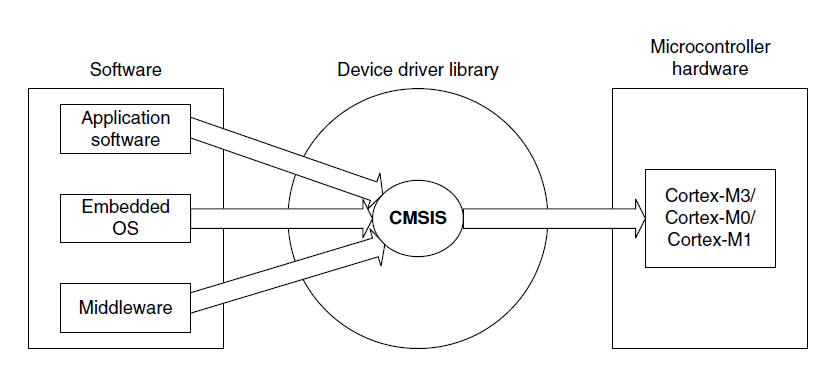
\includegraphics[width=4in]{figure/CMSIS1}}
\caption[Role of CMSIS]{Role of CMSIS\cite{yiu2009definitive}} 
\label{fig_cmsis1}
\end{figure}

The CMSIS uses standardized methods to organize header files that makes it easy to learn new Cortex-M microcontroller products and improve software portability. With the \verb|<device>.h| (e.g. \verb|LPC17xx.h|) and 
system startup code files (e.g., \verb|startup_LPC17xx.s|), 
your program has a common way to access 

\begin{itemize}
    \item {\bf Cortex-M processor core registers} with standardized definitions for NVIC, SysTick, MPU registers, System Control Block registers , and their core access functions (see $\mathtt{core\_cm\ast.[ch]}$ files). 
    \item {\bf system exceptions} with standardized exception number and handler names to allow RTOS and middleware components to utilize system exceptions without having compatibility issues.
    \item {\bf intrinsic functions with standardized name} to produce instructions that cannot  be generated by IEC/ISO C. 
    \item {\bf system initialization} by common methods for each MCU. Fore example, the standardized $\mathtt{SystemInit()}$ function to configure clock.
    \item {\bf system clock frequency} with standardized variable named as $\mathtt{SystemFrequency}$ defined in the device driver.
    \item {\bf vendor peripherals} with standardized C structure. 
\end{itemize}
%\begin{itemize}
%\item {\bf Core Peripheral Access Layer} provides name definitions, address definitions, and helper functions to access Cortex-M core registers and peripherals such NVIC and MPU.
%\item {\bf Device Peripheral Access Layer (MCU specific)} offers name definitions, address definitions and driver code to access peripherals 
%\end{itemize}
\begin{figure}[ht]
\centerline{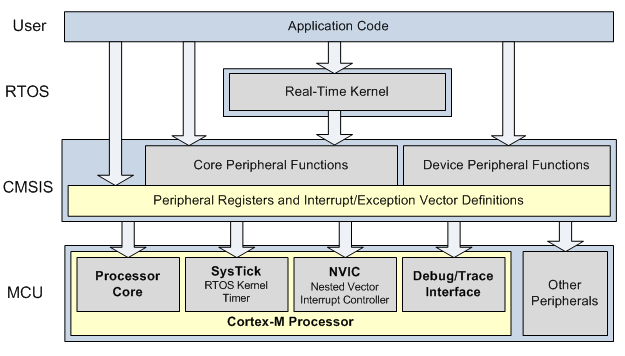
\includegraphics[width=5in]{figure/CMSIS2}}
\caption[CMSIS Organization]{CMSIS Organization\cite{keil.mdk.primer}} 
\label{fig_cmsis2}
\end{figure}

\subsection{CMSIS files} 
The CMSIS is divided into multiple layers (See Figure \ref{fig_cmsis2}). 
For each device, the MCU vendor provides a device header file 
\verb|<device>.h| (e.g., \verb|LPC17xx.h|) which pulls in
additional header files required by the device driver library and 
the Core Peripheral Access Layer (see Figure \ref{fig_cmsis_file_org}).

\begin{figure}[ht]
\centerline{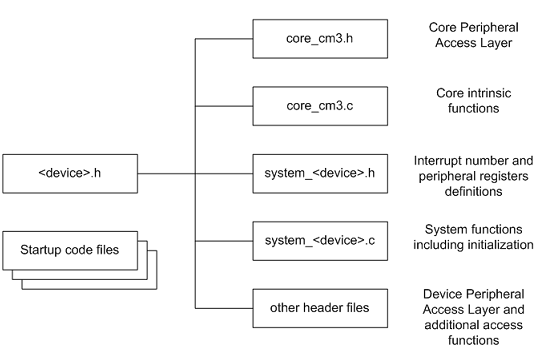
\includegraphics[width=5in]{figure/CMSIS_file_org}}
\caption[CMSIS Organization]{CMSIS Organization\cite{keil.mdk.primer}} 
\label{fig_cmsis_file_org}
\end{figure}

By including the \verb|<device>.h| (e.g., \verb|LPC17xx.h|)  file into 
your code file. The first step to initialize the system 
can be done by calling the CMSIS function as shown in Listing \ref{lst-cmsis-sysinit}.


\begin{lstlisting}[language=C, caption={CMSIS SystemInit()}, label=lst-cmsis-sysinit]
SystemInit();   // Initialize the MCU clock
\end{lstlisting}

The CMSIS compliant device drivers also contain a startup code 
(e.g., \verb|startup_LPC17xx.s|), which include the vector table 
with standardized exception handler names (See Section \ref{sec_exception}.

\subsection{Cortex-M Core Peripherals}
We only introduce the NVIC programming in this section. 
The Nested Vectored Interrupt Controller (NVIC) can be accessed by using CMSIS functions (see Figure \ref{fig_cmsis_nvic}).
\begin{figure}[ht!]
\centerline{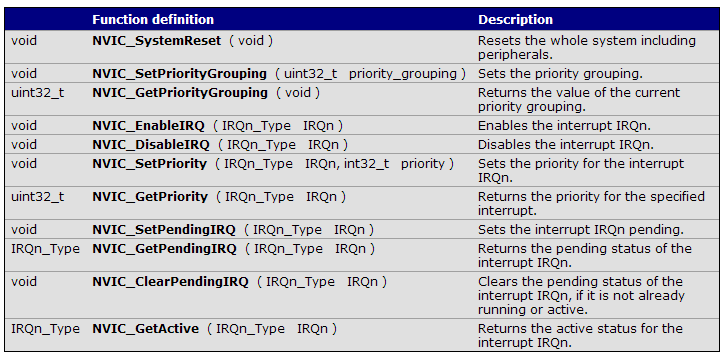
\includegraphics[width=5.5in]{figure/CMSIS_nvic}}
\caption[CMSIS NVIC Functions]{CMSIS NVIC Functions\cite{keil.mdk.primer}} 
\label{fig_cmsis_nvic}
\end{figure}
As an example, the following code enables the UART0 and TIMER0 interrupt 
\begin{lstlisting}[language=C]
NVIC_EnableIRQ(UART0_IRQn);   // UART0_IRQn is defined in LPC17xx.h
NVIC_EnableIRQ(TIMER0_IRQn);  // TIMER0_IRQn is defined in LPC17xx.h
\end{lstlisting}

\subsection{System Exceptions}
\label{sec_exception}
Writing an exception handler becomes very easy. One just defines a function that takes no input parameter and returns void. The function takes the name of the standardized exception handler name as defined in the startup code (e.g., \verb|startup_LPC17xx.s|). The following listing shows an example to write the UART0 interrupt handler entirely in C. \\
\begin{lstlisting}[language=C]
void UART0_Handler (void) 
{
    // write your IRQ here
}
\end{lstlisting}

\clearpage
Another way is to use the embedded assembly code: \\
\begin{lstlisting}[style=asm]
__asm void UART0_Handler(void)
{
    ; do some asm instructions here
    BL __cpp(a_c_function) ; a_c_function is a regular C function
    ; do some asm instructions here, 
}
\end{lstlisting}

\subsection{Intrinsic Functions}

ANSI cannot directly access some Cortex-M3 instructions. The CMSIS provides
intrinsic functions that can generate these instructions. The CMSIS also provides a number of functions for accessing the special registers using $\mathtt{MRS}$ and $\mathtt{MSR}$ instructions. The intrinsic functions are provided by the RealView Compiler.  Table \ref{tb_intrinsic_func} lists some intrinsic functions that your RTOS project most likely will need to use. 
We refer the reader to Tables $613$ and $614$ one page $650$ in Section 34.2.2 of \cite{nxp.lpc17xx.manual} for the complete list of intrinsic functions. 
\begin{table}
\begin{center}
\begin{tabular}{lll}
\hline
Instruction & & CMSIS Intrinsic Function \\ \hline
$\mathtt{CPSIE~ I}$ &   & $\mathtt{void~ \_\_enable\_irq(void)}$ \\
$\mathtt{CPSID~ I}$ &   & $\mathtt{void~ \_\_disable\_irq(void)}$ \\ 
\hline \hline 
Special Register & Access & CMSIS Function \\ \hline
CONTROL      & Read   & $\mathtt{uinit32\_t~ \_\_get\_CONTROL(void)}$ \\
             & Write  & $\mathtt{void~ \_\_set\_CONTROL(uint32\_t~ value})$\\
\hline
MSP          & Read   & $\mathtt{uinit32\_t~ \_\_get\_MSP(void)}$ \\
             & Write  & $\mathtt{void~ \_\_set\_MSP(uint32\_t~ value})$\\
\hline
PSP          & Read   & $\mathtt{uinit32\_t~ \_\_get\_PSP(void)}$ \\
             & Write  & $\mathtt{void~ \_\_set\_PSP(uint32\_t~ value})$\\
\hline
\end{tabular}
\caption[CMSIS intrinsic functions]
        {CMSIS intrinsic functions defined in $\mathtt{core\_cmFunc.h}$}
\label{tb_intrinsic_func}
\end{center}
\end{table}

\subsection{Vendor Peripherals}
All vendor peripherals are organized as C structure in the 
\verb|<device>.h| file (e.g., \verb|LPC17xx.h|). For example, to read
a character received in the RBR of UART0, we can use the following code. 
\begin{lstlisting}[language=C]
unsigned char ch;
ch = LPC_UART0->RBR; // read UART0 RBR and save it in ch  
\end{lstlisting}

\section{Accessing C Symbols from Assembly}
\label{sec_asm_c}
Only embedded assembly is support in Cortex-M3. To write an embedded assembly function, you need to use the $\mathtt{\_\_asm}$ keyword. For example the the function ``$\mathtt{embedded\_asm\_function}$" in Listing \ref{lst_asm_gvar} is an embedded assembly function. You can only put assembly instructions inside this function. Note that inline assembly is not supported in Cortex-M3.

The $\mathtt{\_\_cpp}$ keyword allows one to access C compile-time constant expressions, including the addresses of data or functions with external linkage, from the assembly code. The expression inside the $\mathtt{\_\_cpp}$ can be one of the followings:
\begin{itemize}
\item A global variable defined in C. In Listing \ref{lst_c_gvar}, we have two C global variables \verb+g_pcb+ and \verb+g_var+. We can use the $\mathtt{\_\_cpp}$ to access them as shown in Listing \ref{lst_asm_gvar}. Note to access the value of a variable, it needs to be a constant variable. For a non-constant variable, the assembly code access the address of the variable.

\begin{lstlisting}[caption={Example of accessing C global variables from assembly. The C code.}, label=lst_c_gvar]
#define U32 unsigned int 
#define SP_OFFSET 4

typedef struct pcb {
    struct pcb *mp_next;
    U32 *mp_sp; // 4 bytes offset from the starting address of
                // this structure
    //other variables...
} PCB;

PCB g_pcb;
const U32 g_var;
\end{lstlisting}


\begin{lstlisting}[style=asm, caption={Example of accessing global variable from assembly}, label=lst_asm_gvar]
__asm embedded_asm_function(void) { 
    LDR R3, =__cpp(&g_pcb)   ; load R3 with the address of g_pcb
    LDM R3, {R1, R2}         ; load R1 with g_pcb.mp_next
                             ; load R2 with g_pcb.mp_sp
    LDR R4, =__cpp(g_var)    ; load R4 with the value of g_var, which is a constant
    STR R4, [R3, #SP_OFFSET] ; write R4 value to g_pcb.mp_sp
}
\end{lstlisting}
\item A C function. In Listing \ref{lst_asm_cfunc}, \verb+a_c_function+ is a function written in C. We can invoke this function by using the assembly language. 
\begin{lstlisting}[style=asm, caption={Example of accessing c function from assembly}, label=lst_asm_cfunc]
extern void a_c_function(void);
...
__asm embedded_asm_function(void) {
    ;......
    BL __cpp(a_c_function) ; a_c_function is regular C function
    ;......
}
\end{lstlisting}
\item A constant expression in the range of $0-255$ defined in C. In Listing \ref{lst_asm_gconst}, \verb+g_flag+ is such a constant. We can use $\mathtt{MOV}$ instruction on it. 
Note the $\mathtt{MOV}$ instruction only applies to immediate constant value in the range of $0-255$. 
\begin{lstlisting}[style=asm, caption={Example of accessing constant from assembly}, label=lst_asm_gconst]
unsigned char const g_flag;

__asm embedded_asm_function(void) {
    ;......
    MOV R4, #__cpp(g_flag) ; load g_flag value into R4
    ;......
}
\end{lstlisting}
\end{itemize}

You can also use the \verb|IMPORT| directive to import a C symbol in the embedded assembly function and then start to use the imported symbol just as a regular assembly symbol (see Listing \ref{lst_asm_import}).
\begin{lstlisting}[style=asm, caption={Example of using IMPORT directive to import a C symbol.}, label=lst_asm_import]
void a_c_function (void) {
   // do something 
}

__asm embedded_asm_add(void) {
    IMPORT a_c_function ; a_c_function is a regular C function
    BL a_c_function     ; branch with link to a_c_function
}
\end{lstlisting}

Names in the \verb|__cpp| expression are looked up in the C context of the \verb|__asm| function. Any names in the result of the \verb|__cpp| expression are mangled as required and automatically have \verb|IMPORT| statements generated from them.

\section{SVC Programming: Writing an RTX API Function}
\label{sec_svc}
\begin{figure}[ht]
\centerline{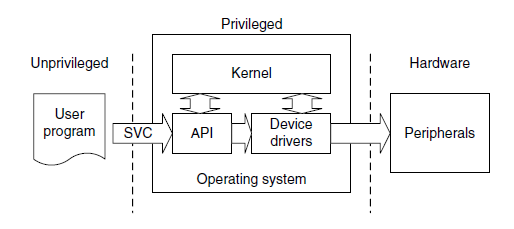
\includegraphics[width=4in]{figure/svc_gateway}}
\caption {SVC as a Gateway for OS Functions \cite{yiu2009definitive}}
\label{fig_svc_gateway}
\end{figure}
A function in RTX API requires a service from the operating system. It needs to be implemented through the proper gateway by {\em trapping} from the user level into the kernel level. On Cortex-M3, the \verb+SVC+ instruction is used to achieve this purpose.  

The basic idea is that when a function in RTX API is called from the user level, this function will trigger an \verb+SVC+ instruction. The \verb+SVC_Handler+, which is the CMSIS standardized exception handler for \verb+SVC+ exception will then invoke the kernel function that provides the actual service (see Figure \ref{fig_svc_gateway}). Effectively, the RTX API function is a wrapper that invokes \verb+SVC+ exception handler and passes corresponding kernel service operation information to the SVC handler.

To generate an SVC instruction, there are two methods. One is a direct method and the other one is an indirect method. 

The direct method is to program at assembly instruction level. We can use the embedded assembly mechanism and write \verb+SVC+ assembly instruction inside the embedded assembly function. An example implementation of
is shown in
Listing \ref{lst-release-memory-block} shows an example implementation of \verb+int release_memory_block(void *memory_block)+. 
\begin{lstlisting}[caption={Code Snippet of release\_memory\_block}, label=lst-release-memory-block]
__asm int release_memory_block(void *memory_block) {
    LDR  R12,=__cpp(k_release_memory_block)
    ; privileged mode code handling omitted 
    SVC  0
    BX   LR
    ALIGN
}
\end{lstlisting}
The corresponding kernel function is the C function \verb+k_release_memory_block+. This function entry point is loaded to \verb+r12+. Then  \verb+SVC 0+ causes an SVC exception with immediate number \verb+0+.
In the SVC exception handler, we can then branch with link and exchange to the address stored in \verb+r12+. Listing \ref{lst-svc_handler} is an excerpt of the \verb+SVC_handler+ in \verb+HAL.c+ from the starter code (\url{https://github.com/yqh/SE350/blob/master/manual_code/SVC/src/HAL.c}).

\begin{lstlisting}[caption={Code Snippet of SVC\_Handler}, label=lst-svc_handler]
  __asm void SVC_Handler(void) {
    
    ; extract SVC number, if it 0, then extract R12 from the exception stack frame
    ; save cpu registers

    BLX  R12 ; R12 contains the kernel function entry point

    ; store C kernel function return value in R0 to R0 on the exception stack frame omitted
    ; restore cpu registers
}
\end{lstlisting}
%write more about each line here, no time to finish for now

The indirect method is to ask the compiler to generate the \verb+SVC+ instruction from C code. The ARM compiler provides an intrinsic keyword named \verb+__svc_indirect+ which passes an operation code to the SVC handler in \verb+r12+\cite{arm.rvct.comp.ref}. This keyword is a function qualifier. The two inputs we need to provide to the compiler are
\begin{itemize}
\item \verb+svc_num+, the immediate value used in the \verb+SVC+ instruction and
\item \verb+op_num+, the value passed in \verb+r12+ to the handler to determine the function to perform. The following is the syntax of an indirect SVC. 
\end{itemize}
\begin{lstlisting}
__svc_indirect(int svc_num)
        return_type function_name(int op_num[, argument-list]);
\end{lstlisting}
The system handler must make use of the \verb+r12+ value to select the required operation. For example, the \verb+release_memory_block+ is a user function with the following signature:
\begin{lstlisting}
#include <rtx.h>
int release_memory_block(void *memory_block);
\end{lstlisting}
In \verb+rtx.h+, the following code is revelent to the implementation of the function.
\begin{lstlisting}
#define __SVC_0 __svc_indirect(0)
extern int k_release_memory_block(void *);
#define release_memory_block(p_mem_blk) _release_memory_block((U32)k_release_memory_block, p_mem_blk)
extern int _release_memory_block(U32 p_func, void *p_mem_blk) __SVC_0;
\end{lstlisting}
The compiler generates two assembly instructions
\begin{lstlisting}
    LDR.W r12, [pc, #offset]; Load k_release_memory_block in r12
    SVC 0x00
\end{lstlisting}
The \verb+SVC_handler+ in Listing \ref{lst-svc_handler} then can be used to handle the \verb+SVC 0+ exception.
% TOdo: can explain more here, no time for now to do so

\section{UART Programming}
\label{sec_uart_programming}

The ultimate reference of LPC1768 UART is chapters 15 and 16 of \cite{nxp.lpc17xx.manual}. There are four UARTs on the chip. We use UART0 and UART1. The UART data transmission can be interrupt driven or polled. In this project, we configure UART0 to be interrupt driven for both receiving and transmitting. UART1 is configured to use polling for both data receiving and transmitting. 

The LPC1768 UART receiver and transmitter have a 16-element FIFO each and they are referred as RX FIFO and TX FIFO respectively. The Receiver Buffer Register (RBR) is the top byte (i.e. the oldest byte) of the RX FIFO. The Transmit Holding Register (THR) is the top byte (i.e. the newest byte) of the TX FIFO. To write to the THR, one needs to make sure the THR is empty. Otherwise, the write will overwrite the byte in THR which is not shifted out by the transmit shift register. When programming the UART by polling, one can poll the status bits in the Line Status Register (LSR). When programming the UART as interrupt-driven, the interrupt is the FIFO status indicator. 

To program a UART on MCB1700 board, one first needs to configure the UART by following the steps listed in Section 15.1 in \cite{nxp.lpc17xx.manual} (referred as LPC17xx\_UM in the sample code comments). 
Listings \ref{lst-uart-def-h}, \ref{lst-uart-irq-h} \ref{lst-uart-irq-c}, and \ref{lst-main-uart-irq-c} give one possible implementation of programming UART0 interrupts.
This implementation configures the RX FIFO interrupt to be triggered when one character is received by the RX FIFO. The transmit interrupt is triggered when the transmit holding register becomes empty.
The RX FIFO interrupt is always on and the TX FIFO interrupt is turned off when there are no data to transmit by the interrupt handler and turned back on when there are data to transmit by the main program. The UART Interrupt Enable Register (IER) controls the UART device level interrupt source setting. \\

\lstinputlisting[language=C, caption={UART0 IRQ Code uart\_def.h}, label=lst-uart-def-h]{code/uart_def.h}
\lstinputlisting[language=C, caption={UART0 IRQ Code uart\_irq.h}, label=lst-uart-irq-h]{code/uart_irq.h}
\lstinputlisting[language=C, caption={UART0 IRQ Code uart\_irq.c}, label=lst-uart-irq-c]{code/uart_irq.c}
\lstinputlisting[language=C, caption={UART0 IRQ Code main\_uart\_irq.c}, label=lst-main-uart-irq-c]{code/main_uart_irq.c}

Listings 
\ref{lst-uart-polling-h} and \ref{lst-uart-polling-c} give one sample implementation of programming UART0 by polling.
\lstinputlisting[language=C, caption={UART0 Polling Code uart\_polling.h}, label=lst-uart-polling-h]{code/uart_polling.h}
\lstinputlisting[language=C, caption={UART0 Polling Code uart\_polling.c}, label=lst-uart-polling-c]{code/uart_polling.c}
%\lstinputlisting[language=C, caption={UART0 Polling Code main\_uart\_polling.c}, label=lst-main-uart-polling-c]{code/main_uart_polling.c}

\section{Timer Programming}
To program a TIMER on MCB1700 board, one first needs to configure the TIMER by following the steps listed in Section 21.1 in \cite{nxp.lpc17xx.manual}. Listings \ref{lst-timer-irq-h} and \ref{lst-timer-irq-c} give one sample implementation of programming TIMER0 interrupts. The timer interrupt fires every one millisecond. 
\\
\lstinputlisting[language=C, caption={Timer0 IRQ Sample Code timer.h}, label=lst-timer-irq-h]{code/timer.h}
\lstinputlisting[language=C, caption={Timer0 IRQ Sample Code timer.c}, label=lst-timer-irq-c]{code/timer.c}

%write about free list for memory management inlcuding scatter file
%defined symbol $$.. to indicate end of image

%section{Memory Protection Unit Programming}

%%% Local Variables:
%%% mode: latex
%%% TeX-master: "main_book"
%%% End:
